%%%%%%%%%%%%%%%%%%%%%%%%%%%%%%%%%%%%%%%%%%%%%%%%%%%%%%%%%%%%%%%%%%%%%%
% amspaper.tex --  LaTeX2e-based template for submissions to American 
% Meteorological Society Journals, including
%
% JAS 	-- Journal of the Atmospheric Sciences
% JAMC 	-- Journal of Applied Meteorology and Climatology
% JPO 	-- Journal of Physical Oceanography
% MWR 	-- Monthly Weather Review
% JTECH -- Journal of Atmospheric and Oceanic Technology
% WAF 	-- Weather and Forecasting
% JCLI 	-- Journal of Climate
% JHM 	-- Journal of Hydrometeorology
% JAM 	-- Journal of Applied Meteorology
%
% Template developed by B. Papa and S. Cooley, AMS. 
% Email questions to latex@ametsoc.org.
%
% August 12, 2008 (SRC)
%	- Clarified/added header notes, comments throughout
%	- Improved title page
%	- Edited text of document for clarity
%	- Altered list styles to adhere to AMS style, added comments
%	- Removed incorrect commands (i.e., \catcode) (corrects umlaut bug)
%	- Moved non-template commands to ametsoc.sty
%
% August, 2008 - B. Papa
% - Updated to handle two column journal page output
% - Updated text with new/modified instructions
%
%%%%%%%%%%%%%%%%%%%%%%%%%%%%%%%%%%%%%%%%%%%%%%%%%%%%%%%%%%%%%%%%     
%%%%%%%%%%%%%%%%%%%%%%%%%%%%%%%%%%%%%%%%%%%%%%%%%%%%%%%%%%%%%%%%
%																															 %
%				USE THIS TEMPLATE, AMETSOC.STY, AND AMETSOC.BST				 %
%			        OR YOUR TEX FILES WILL NOT BE USED				  		 %
%																															 % 
%%%%%%%%%%%%%%%%%%%%%%%%%%%%%%%%%%%%%%%%%%%%%%%%%%%%%%%%%%%%%%%%
%%%%%%%%%%%%%%%%%%%%%%%%%%%%%%%%%%%%%%%%%%%%%%%%%%%%%%%%%%%%%%%%

%%%%%%%%%%%%%%%%%%%%%%%%%%%%%%%%%%%%%%%%%%%%%%%%%%%%%%%%%%%%%%%%%%%%%
% PREAMBLE
%%%%%%%%%%%%%%%%%%%%%%%%%%%%%%%%%%%%%%%%%%%%%%%%%%%%%%%%%%%%%%%%%%%%%
%
% The following two commands will generate a PDF that follows all the requirements for submission
% and peer review.  Uncomment these commands to generate this output (and comment out the two lines below.)
%
% DOUBLE SPACE VERSION FOR SUBMISSION TO THE AMS
\documentclass[12pt]{article}
\usepackage{ametsoc}
%
% The following two commands will generate a single space, double column paper that closely
% matches an AMS journal page.  Uncomment these commands to generate this output (and comment
% out the two lines above. FOR AUTHOR USE ONLY. PAPERS SUBMITTED IN THIS FORMAT WILL BE RETURNED
% TO THE AUTHOR for submission with the correct formatting.
%
% TWO COLUMN JOURNAL PAGE LAYOUT FOR AUTHOR USE ONLY
%\documentclass[10pt]{article}
%\usepackage{ametsoc2col}
\usepackage{subfigure}
%
%%%%%%%%%%%%%%%%%%%%%%%%%%%%%%%%%%%%%%%%%%%%%%%%%%%%%%%%%%%%%%%%%%%%%
% ABSTRACT
%
% Enter your Abstract here
%%%%%%%%%%%%%%%%%%%%%%%%%%%%%%%%%%%%%%%%%%%%%%%%%%%%%%%%%%%%%%%%%%%%%
\newcommand{\myabstract}{The Limited Area Model (LAM) forecasting problem is a lateral boundary 
condition problem in addition to the initial condition problem. For 
numerical weather prediction, the lateral boundary conditions are generally 
provided by a host model, for example a global numerical weather prediction 
model. One may argue that the available boundary conditions from the host 
model have to be accepted (without change) for usage in the LAM. However, 
one may use the observations close to the lateral boundaries and let these 
influence the initial conditions. In case the initial conditions are used as the 
lateral boundary conditions at the initial time, the subsequent forecast will 
also be influenced by these observations. Depending on the frequency of the 
updating of the lateral boundary conditions, the host model will gradually 
take over the definition of the lateral boundary conditions. With application of
 4D-Var for the LAM forecasting, one could do a bit more, since one 
may control the lateral boundary conditions during the period of the data 
assimilation window. This may be particularly important for assimilation of 
phenomena that are observed well inside the LAM domain during the later 
part of the data assimilation window, while being propagated through the 
lateral boundaries during the early part of the data assimilation window. 
If we do not control the lateral boundary conditions, observed information 
related to these phenomena may be lost.}
%
\begin{document}
%
%%%%%%%%%%%%%%%%%%%%%%%%%%%%%%%%%%%%%%%%%%%%%%%%%%%%%%%%%%%%%%%%%%%%%
% TITLE
%
% Enter your TITLE here
%%%%%%%%%%%%%%%%%%%%%%%%%%%%%%%%%%%%%%%%%%%%%%%%%%%%%%%%%%%%%%%%%%%%%
\title{\textbf{\large{Control of lateral boundary conditions in WRF 4D-Var}}}
%
% Author names, with corresponding author information. 
% [Update and move the \thanks{...} block as appropriate.]
%
\author{\textsc{Xin Zhang}
             \textsc{and Xiang-Yu Huang}
				\thanks{\textit{Corresponding author address:} 
				Dr. Xiang-Yu Huang, NCAR/MMM, P.O. Box 3000, 
				 Boulder, CO 80307. 
				\newline{E-mail: huangx@ucar.edu}}\\
\textit{\footnotesize{MMM, National Center for Atmospheric Research, Boulder, CO 80305}}
\and 
\centerline{\textsc{Nils Gustafsson}}\\% Add additional authors, different insitution
\centerline{\textit{\footnotesize{Swedish Meteorological and Hydrological Institute, SE-60176 Norrk�oping, Sweden}}}
}
%
% The following block of code will handle the formatting of the title page depnding on whether
% we are formatting a double column (dc) author draft or a single column paper for submission.
% AUTHORS SHOULD SKIP OVER THIS... There is nothing to do in this section of code.
\ifthenelse{\boolean{dc}}
{
\twocolumn[
\begin{@twocolumnfalse}
\amstitle

% Start Abstract (Enter your Abstract above.  Do not enter any text here)
\begin{center}
\begin{minipage}{13.0cm}
\begin{abstract}
	\myabstract
	\newline
	\begin{center}
		\rule{38mm}{0.2mm}
	\end{center}
\end{abstract}
\end{minipage}
\end{center}
\end{@twocolumnfalse}
]
}
{
\amstitle
\begin{abstract}
\myabstract
\end{abstract}
\newpage
}
%%%%%%%%%%%%%%%%%%%%%%%%%%%%%%%%%%%%%%%%%%%%%%%%%%%%%%%%%%%%%%%%%%%%%
% MAIN BODY OF PAPER
%%%%%%%%%%%%%%%%%%%%%%%%%%%%%%%%%%%%%%%%%%%%%%%%%%%%%%%%%%%%%%%%%%%%%
%
\section{Background}
For the control of lateral boundary conditions in WRF 4D-Var, we follow \cite{Kawa2007} and we introduce the lateral boundary condition perturbations as a control variable $\delta{\mathbf{x}_\mathrm{lbc}}(t_k)$  at the end of the data assimilation window (time $t_k$).  For the lateral boundary increment $\delta{\mathbf{x}_\mathrm{lbc}}(t_0)$ at the start of the assimilation window (time $t_0$) we will use the initial condition increment $\delta{\mathbf{x}}(t_0)$. For intermediate time-steps during the integration of the tangent linear model, we will obtain the lateral boundary conditions by the same linear time interpolation scheme that is used in the non-linear model. Once the lateral boundary conditions are defined, the same lateral boundary relaxation scheme, see \cite{Davis1983}, that is used in the non-linear model can also be used in the tangent-linear model, and the adjoint of the lateral 
boundary relaxation is also well defined, see \cite{Gusta1998}. Note however, that while the lateral boundary conditions are input data to the tangent linear model, the lateral boundary conditions are output data from 
the adjoint model. 

Again following \cite{Kawa2007} we will introduce a cost function term $J_\mathrm{lbc}$ that will measure the distance to the un-perturbed lateral boundary conditions used in the non-linear model 
\begin{equation}
J_\mathrm{lbc}=(\delta{\mathbf{x}_\mathrm{lbc}}(t_k))^T\bm{\mathsf{B}}_\mathrm{lbc}^{-1}\delta{\mathbf{x}_\mathrm{lbc}}(t_k)
\end{equation}
where $\bm{\mathsf{B}}_\mathrm{lbc}$ represents the covariance of the lateral boundary condition 
errors. Lateral boundary conditions only need to be defined in the narrow 
lateral boundary relaxation zone, but obviously it would be difficult to specify the proper spatial scales and balances representing the lateral boundary condition errors over such a narrow domain. We have therefore made the 
choice to specify the lateral boundary control variable over the same total
 model domain as the initial condition control variable. Since both of 
these control variables represent forecast errors, albeit for different forecast 
lengths and possibly for different models, it is clear that their respective 
error covariance can be represented in a similar way. In a first trial to test 
the sensitivity of the assimilation to the control of the lateral boundary 
conditions, we will simply apply $\bm{\mathsf{B}}_\mathrm{lbc}=\bm{\mathsf{B}}$. 

One potential problem is that the introduction of the lateral boundary 
condition constraint in the form described above, would worsen the conditioning of the 4D-Var minimization problem, since the lateral boundary condition errors at the end of the assimilation window would be strongly 
correlated with the initial condition errors at the start of the assimilation 
window, at least for the large scale and slowly varying phenomena that are 
important for the lateral boundary conditions. One simple pre-conditioning 
would be to subtract the lateral boundary conditions at the start of the 
assimilation window from the lateral boundary conditions at the end of 
the assimilation window, thus to treat the tendency of the lateral boundary 
conditions 
\begin{displaymath}
(\frac{\partial{\delta{\mathbf{x}_\mathrm{lbc}}}}{\partial{t}})=\frac{\delta{\mathbf{x}_\mathrm{lbc}}(t_k)-\delta{\mathbf{x}_\mathrm{lbc}}(t_0)} {t_{k}-t_0}
\end{displaymath}
as the control variable. This approach would also require the covariance of forecast tendency errors, that possibly 
could be estimated by the NMC method from differences between forecast 
tendencies valid at the same time. 

\section{Formulation}
A similar control of lateral boundary condition as developed for HIRLAM 
4D-Var will be developed also for the WRF 4D-Var. As a starting point, the 
lateral boundary conditions at the end of the data assimilation window will
be used as the control variable. The main difference between the implementation in WRF 4D-Var and HIRLAM 4D-Var is due to the differences between 
the lateral boundary relaxation schemes, where the WRF uses a boundary 
relaxation applied in a �nudging� of model tendencies, following \cite{Davis1977}
\begin{equation}
\frac{\partial{\mathbf{x}}}{\partial{t}}=F_1(\mathbf{x}_\mathrm{lbc}-\mathbf{x})-F_2\Delta^2(\mathbf{x}_\mathrm{lbc}-\mathbf{x})
\end{equation}
where $\Delta^2$ is a 5-point smoothing operator,$ F_1$ and $F_2$ are (nudging) 
weighting coefficients depending on the distance to the lateral boundary, $\mathbf{x}$ 
is any model state variable and $\mathbf{x}_\mathrm{lbc}$ is the corresponding boundary value 
provided by the host model. $\mathbf{x}_\mathrm{lbc}$ is speci�ed in the following form:
\begin{equation}
\mathbf{x}_\mathrm{lbc}(time=t)=\mathbf{x}_\mathrm{lbc}(time=t_0)+(t-t_0)\frac{\partial{\mathbf{x}_\mathrm{lbc}}}{\partial{t}}
\end{equation}
Considering a data assimilation window from time $t_0$ until time $t_k$ and 
having $\delta{\mathbf{x}}(t_0)$ and $\delta{\mathbf{x}_\mathrm{lbc}}(t_k)$ as the assimilation control variables, the quantities needed for the LBC of the tangent linear WRF model are given by
\begin{equation}
\delta{\mathbf{x}}_\mathrm{lbc}(t_0)=\delta{\mathbf{x}}(t_0)
\end{equation}
\begin{equation}
\frac {\partial{\delta{\mathbf{x}}_\mathrm{lbc}}} {\partial{t}}=\frac{\delta{\mathbf{x}}_\mathrm{lbc}(t_k)-\delta{\mathbf{x}}(t_0)} {t_k-t_0}
\end{equation}
The lateral boundary conditions for the adjoint model, $\mathbf{x}_\mathrm{lbc}^\mathrm{AD}(t_0)$ and $(\frac {\partial{\mathbf{x}}_\mathrm{lbc}} {\partial{t}})^\mathrm{AD}$
, will be initialized with zeroes at the end of the data assimilation 
window (time $t_k$ ). After the backwards integration of the adjoint model to 
time $t_0$ the adjoint control variables (or the error gradients) can be obtained 
from: 
\begin{equation}
\mathbf{x}^\mathrm{AD}(t_0)=\mathbf{x}_\mathrm{inner}^\mathrm{AD}(t_0)+\mathbf{x}_\mathrm{lbc}^\mathrm{AD}(t_0)-\frac{1.}{t_k-t_0}(\frac{\partial{\mathbf{x}_\mathrm{lbc}}}{\partial{t}})^\mathrm{AD}
\end{equation}
\begin{equation}
\mathbf{x}_\mathrm{lbc}^\mathrm{AD}(t_k)=\frac{1.}{t_k-t_0}(\frac{\partial{\mathbf{x}_{lbc}}}{\partial{t}})^\mathrm{AD}
\end{equation}
where $\mathbf{x}_\mathrm{inner}^\mathrm{AD}(t_0)$ denotes the �inner domain� adjoint model model variable as provided at the initial time $t_0$.

Note that $\mathbf{x}_\mathrm{lbc}^\mathrm{AD}(t_0)$ and $(\frac{\partial{\mathbf{x}_\mathrm{lbc}}}{\partial{t}})^\mathrm{AD}$ will be defined in the boundary relaxtion 
zone only. Consider, however, that they are full domain �elds that were 
initialized with zeroes at the the end of the data assimilation window and that the boundary relaxation will only fill in values into this full domain 
field inside the boundary relaxtion zone.

Also note that the calculation of $J_\mathrm{lbc}$ and $\frac{\partial{J_\mathrm{lbc}}} {\partial{\mathbf{v}_\mathrm{lbc}}}$, where $\mathbf{v}_\mathrm{lbc}$ is the lateral boundary condition control variable in control vector space, will follow exactly the same calculations as for the background error constraint. 

\section{Code modification}
To introduce the new control variable of lateral boundary, we made following code modification in the latest WRFDA repository :
\subsubsection{Add some variables definition for LBC 4DVAR}
\begin{verbatim}
M      var/da/da_control/da_control.f90
M      var/da/da_define_structures/da_define_structures.f90
\end{verbatim}
\subsubsection{Update the output gradient function print out and the subroutine interface}
\begin{verbatim}
M      var/da/da_minimisation/da_calculate_gradj.inc
\end{verbatim}
\subsubsection{Update the output cost function print out}
\begin{verbatim}
M      var/da/da_minimisation/da_calculate_j.inc
\end{verbatim}
\subsubsection{Add calling \textsl{da\_transfer\_xatowrftl\_adj\_lbc} and \textsl{da\_transform\_vtox\_adj}}
\begin{verbatim}
M      var/da/da_minimisation/da_transform_vtoy_adj.inc
\end{verbatim}
\subsubsection{Update the subroutines' interface due to changes}
\begin{verbatim}
M      var/da/da_minimisation/da_minimise_lz.inc
M      var/da/da_minimisation/da_minimise_cg.inc
\end{verbatim}
\subsubsection{Update the USE statements to accomodate the changes}
\begin{verbatim}
M      var/da/da_minimisation/da_minimisation.f90
\end{verbatim}
\subsubsection{Add statements to call \textsl{da\_transform\_vtox} for 6-hour control variables.\\
Add statements to call \textsl{da\_transfer\_xatowrftl\_lbc}}
\begin{verbatim}
M      var/da/da_minimisation/da_transform_vtoy.inc
\end{verbatim}
\subsubsection{Change cv\_size initialization due to $J_\mathrm{lbc}$}
\begin{verbatim}
M      var/da/da_setup_structures/da_setup_cv.inc
\end{verbatim}
\subsubsection{Minor changes to include more namelist variables in USE statement}
\begin{verbatim}
M      var/da/da_setup_structures/da_setup_structures.f90
\end{verbatim}
\subsubsection{Include the new subroutines}
\begin{verbatim}
M      var/da/da_transfer_model/da_transfer_model.f90
\end{verbatim}
\subsubsection{Add calling statement to output \textsl{wrfbdy\_af07}}
\begin{verbatim}
M      var/da/da_transfer_model/da_transfer_wrftltoxa_adj.inc
\end{verbatim}
\subsubsection{Add the adjoint of converting WRFTL variables to analysis increments at boundary}
\begin{verbatim}
M      var/da/da_transfer_model/da_transfer_xatowrftl_adj.inc
\end{verbatim}
\subsubsection{Adjoint of converting 6-hour analysis increments into WRFTL increments}
\begin{verbatim}
A      var/da/da_transfer_model/da_transfer_xatowrftl_adj_lbc.inc
\end{verbatim}
\subsubsection{Convert 6-hour analysis increments into WRFTL increments}
\begin{verbatim}
A      var/da/da_transfer_model/da_transfer_xatowrftl_lbc.inc
\end{verbatim}
\subsubsection{Clean-up}
\begin{verbatim}
M      var/da/da_transfer_model/da_transfer_wrftoxb.inc
\end{verbatim}
\subsubsection{Change the subroutines' interface due to changes happen elsewhere}
\begin{verbatim}
M      var/da/da_test/da_check_vtoy_adjoint.inc
M      var/da/da_minimisation/da_adjoint_sensitivity.inc
M      var/da/da_minimisation/da_sensitivity.inc
\end{verbatim}
\subsubsection{Input \textsl{wrfbdy\_ad01}, which is the output of the adoint model}
\begin{verbatim}
A      var/da/da_main/da_med_initialdata_input_lbc.inc
\end{verbatim}
\subsubsection{Output \textsl{wrfbdy\_af07}, which is the LBC forcing for the adoint model}
\begin{verbatim}
A      var/da/da_main/da_med_initialdata_output_lbc.inc
\end{verbatim}
\subsubsection{Read in \textsl{wrfbdy\_d01} when 4DVAR}
\begin{verbatim}
M      var/da/da_main/da_wrfvar_init2.inc
\end{verbatim}
\subsubsection{Include the new subroutines \textsl{da\_med\_initialdata\_input\_lbc.inc} \\and \textsl{da\_med\_initialdata\_output\_lbc.inc}}
\begin{verbatim}
M      var/da/da_main/da_wrfvar_io.f90
\end{verbatim}
\subsubsection{Add statements to read \textsl{wrfbdy\_ad01} output from adjoint model}
\begin{verbatim}
M      var/da/da_main/da_med_initialdata_input.inc
\end{verbatim}
\subsubsection{Initialize 6-hour $vv$ and $vp$}
\begin{verbatim}
M      var/da/da_main/da_solve.inc
\end{verbatim}
\subsubsection{Add namelist variables to switch on/off LBC control of 4DVAR.\\
Add control variables space: $\mathbf{x6a}$, $\mathbf{vv6}$ and $\mathbf{vp6}$ for 6-hour}
\begin{verbatim}
M      Registry/Registry.wrfvar
\end{verbatim}


\section{Validation with single observation}
\label{sec:single}
Analysis increments due to a single observation produced by a data assimilation system implicitly provide the effective background error covariance matrix $\bm{\mathsf{B}}$ and describe how the tangent linear and adjoint model propagate the observational information , see \cite{Huang2009}. After any new capability for WRF 4D-Var system was developed, the single observation experiment is an effective and clean way to show the impact of the new capability on the analysis.
As in Fig. 3 of \cite{Huang2009}, given a single temperature observation at the end of the time window of 4D-Var, we knew that the 4D-Var increments have a temporal dimension, the increments at 6 h give a graphic representation of the background error covariance matrix at 6 h, transformed by $\bm{\mathsf{MBM}}^T$. The $\bm{\mathsf{M}}$, $\bm{\mathsf{M}}^T$ are the WRF tangent linear and adjoint model respectively. For current WRF 4D-Var version, WRF is a regional model, and both initial condition and boundary condition determine the future trajectory of the model. Specifically, the trajectory of the 5-point boundary relaxation region is also depend on the tendency from lateral boundary condition. Therefore, in the 4D-Var, the observations close to or within the lateral boundary relaxation region should not only impact the initial condition but also the boundary condition.
To illustrate and verify the correctness of the new capability of adding lateral boundary condition (LBC) into the control variable in 4D-Var, we design 2 single observation experiments similar to that in paper \cite{Huang2009}: The first experiment has a single observation at 6 h, which is far from the lateral boundary and the tendency from LBC should have trivial or no impact on the observation location at 6 h, which means assimilating this observation either with or without LBC control should make little/no difference on the analysis at 0 h; The second experiment also has a single observation at 6 h, but close to the lateral boundary and the tendency from LBC should have significant impact on the observation location at 6 h, which means assimilating this observation with or without LBC control should make big difference on the analysis at 0 h.

\subsection{Experiment 1: Single observation far away from the lateral boundary}
We still utilize the case in \cite{Huang2009},  which is a severe winter storm case that occurred at 0000 UTC 25 January 2000. We used a 6-h forecast valid at 0000 UTC 25 January 2000 as the background for both experiments. A single temperature observation at 0600 UTC is placed at $32.5\,^{\circ}\mathrm{N}$, $75\,^{\circ}\mathrm{W}$, the red cross in Fig.~\ref{fig:center_0h}. Fig.~\ref{fig:center_0h} shows the analysis increments due to the 6 h temperature observation with and without LBC control. There are some difference between Fig.~\ref{fig:center_0h} (a) and (b), but they are quite similar and the main responses are located on the upstream of the observation. We integrated the increments forward from 0 hour to 6 hour, Fig.~\ref{fig:center_6h} and Fig.~\ref{fig:center_lbc_6h} show the similar development of the increments without and with LBC control too, which confirm the assumption that the LBC control does not have too much impact on the assimilation of the observation which far away from the LBC during the 4D-Var time window.
\begin{figure}[t]
\subfigure[Without LBC control]{
\noindent\includegraphics[width=19pc, viewport=20 100 600 730, clip]{./figures/center}}
\subfigure[With LBC control]{
\noindent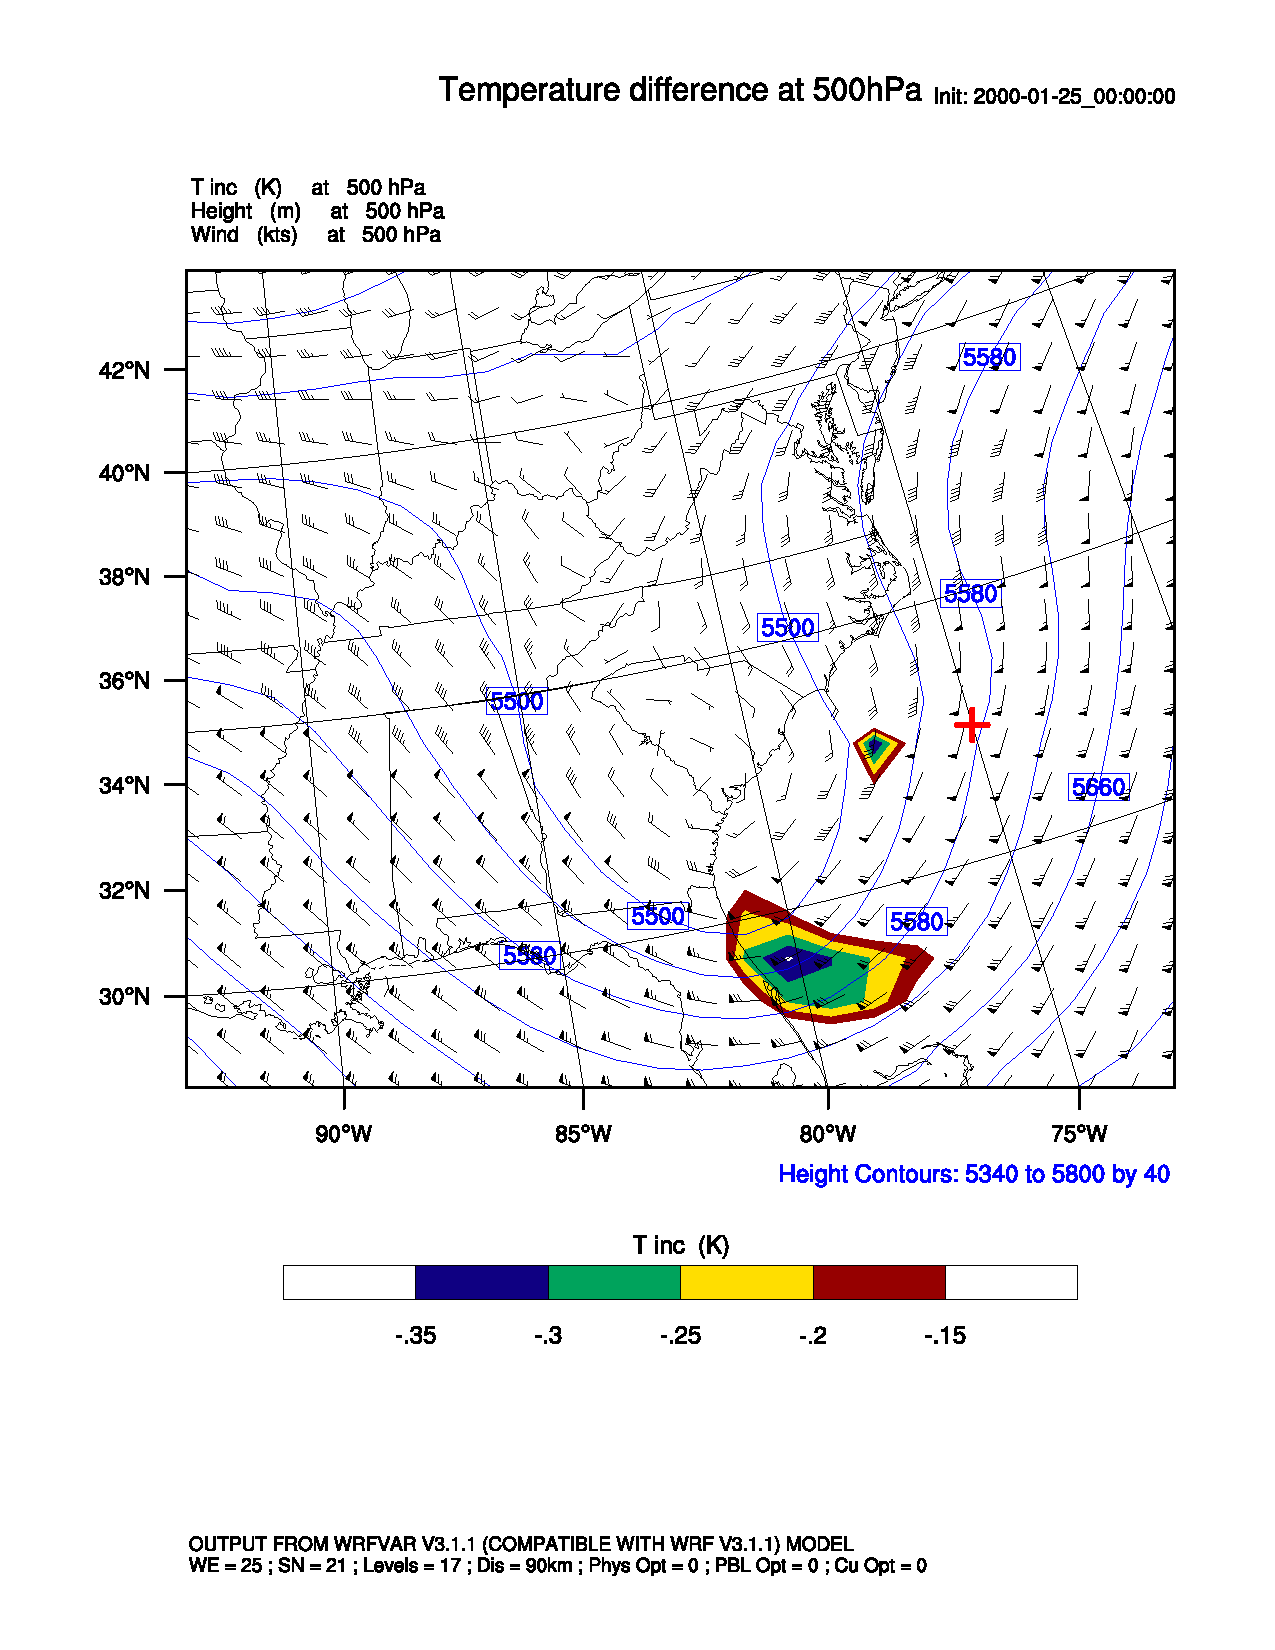
\includegraphics[width=19pc, viewport=20 100 600 730, clip]{./figures/center_lbc}}
\caption{0 hour potential temperature perturbation}\label{fig:center_0h}
\end{figure}

\begin{figure}[t]
\noindent\includegraphics[width=39pc, viewport=20 50 580 750, clip]{./figures/center_6h}
\caption{1-6 hour potential temperature perturbation without LBC control.}\label{fig:center_6h}
\end{figure}
\begin{figure}[t]
\noindent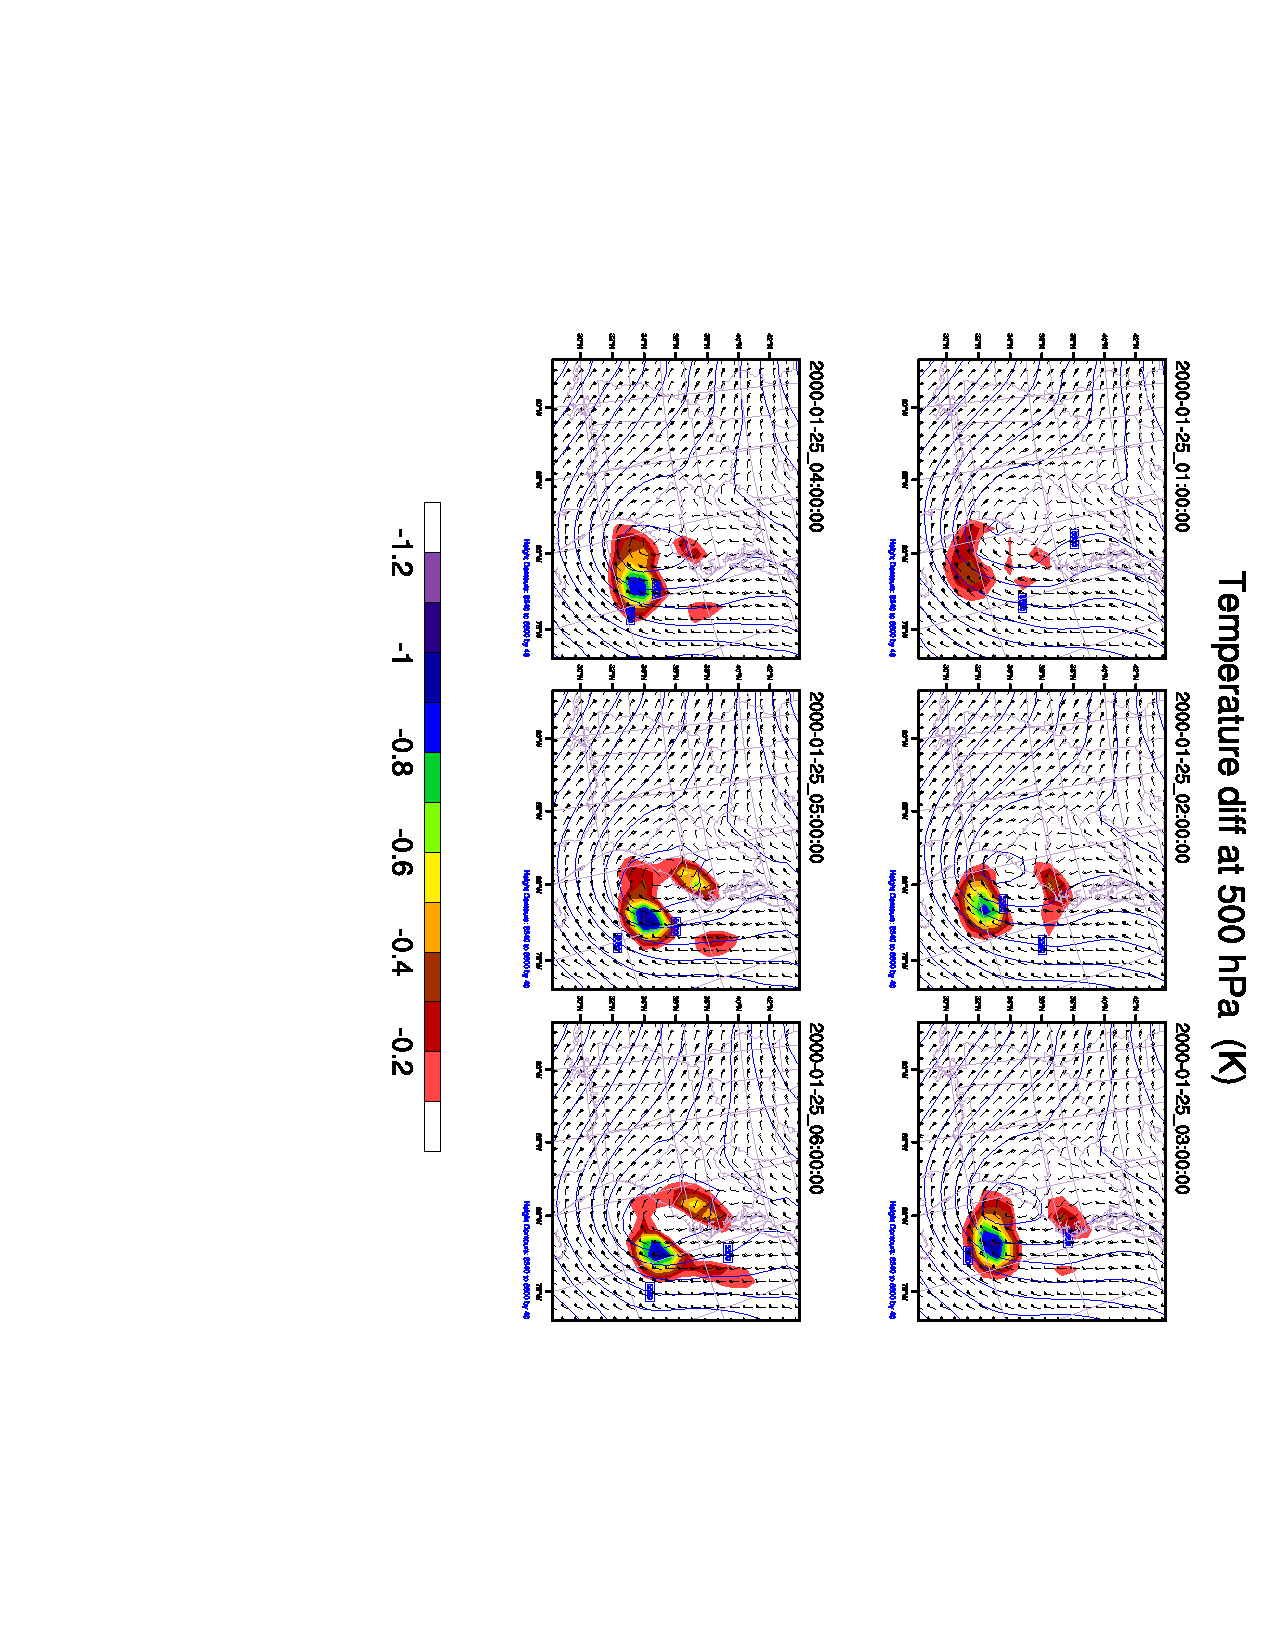
\includegraphics[width=39pc, viewport=20 50 580 750, clip]{./figures/center_lbc_6h}
\caption{1-6 hour potential temperature perturbation with LBC control.}\label{fig:center_lbc_6h}
\end{figure}


\subsection{Experiment 2: Single observation close to the lateral boundary}
We moved the single temperature observation at 0600 UTC to $28\,^{\circ}\mathrm{N}$, $75\,^{\circ}\mathrm{W}$, as the red cross in Fig.~\ref{fig:boundary_0h}. Fig.~\ref{fig:boundary_0h} show the analysis increments due to the 6 h temperature observation with and without LBC control. Because the observation is within the lateral boundary relaxation region, the upstream response of 6 h before should be outside the domain, which means the analysis response at 0 h should be in the tendency of boundary condition. This is the case in Fig.~\ref{fig:boundary_0h}(b), there is no significant response in initial condition when the LBC control was turned on. However, if the LBC control was turned off, then the minimization have to produce some unrealistic or overestimated responses in initial condition to decrease the innovation. That is why some significant responses can be found upstream along the south boundary in Fig.~\ref{fig:boundary_0h}(a).  Then, we integrated the increments forward from 0 hour to 6 hour. The perturbation development in Fig.~\ref{fig:boundary_6h} shows that the original perturbation along south boundary almost doesn't change during the 6 hours, the positive perturbation was developed locally, which means there is no/very few perturbation propagated from LBC tendency. However, in Fig.~\ref{fig:boundary_lbc_6h}, the perturbation along south boundary was developed from scratch and became stronger and stronger, apparently, the LBC tendency did the job. Finally, comparing the increments at 6 h in both figures, we found that the increment in experiment with LBC control fit the observation location much better than that that in the experiment without LBC control. All the results confirm the assumption that the LBC control has significant impact on the assimilation of the observation which close to the LBC during the 4D-Var time window.
\begin{figure}[t]
\subfigure[Without LBC control]{
\noindent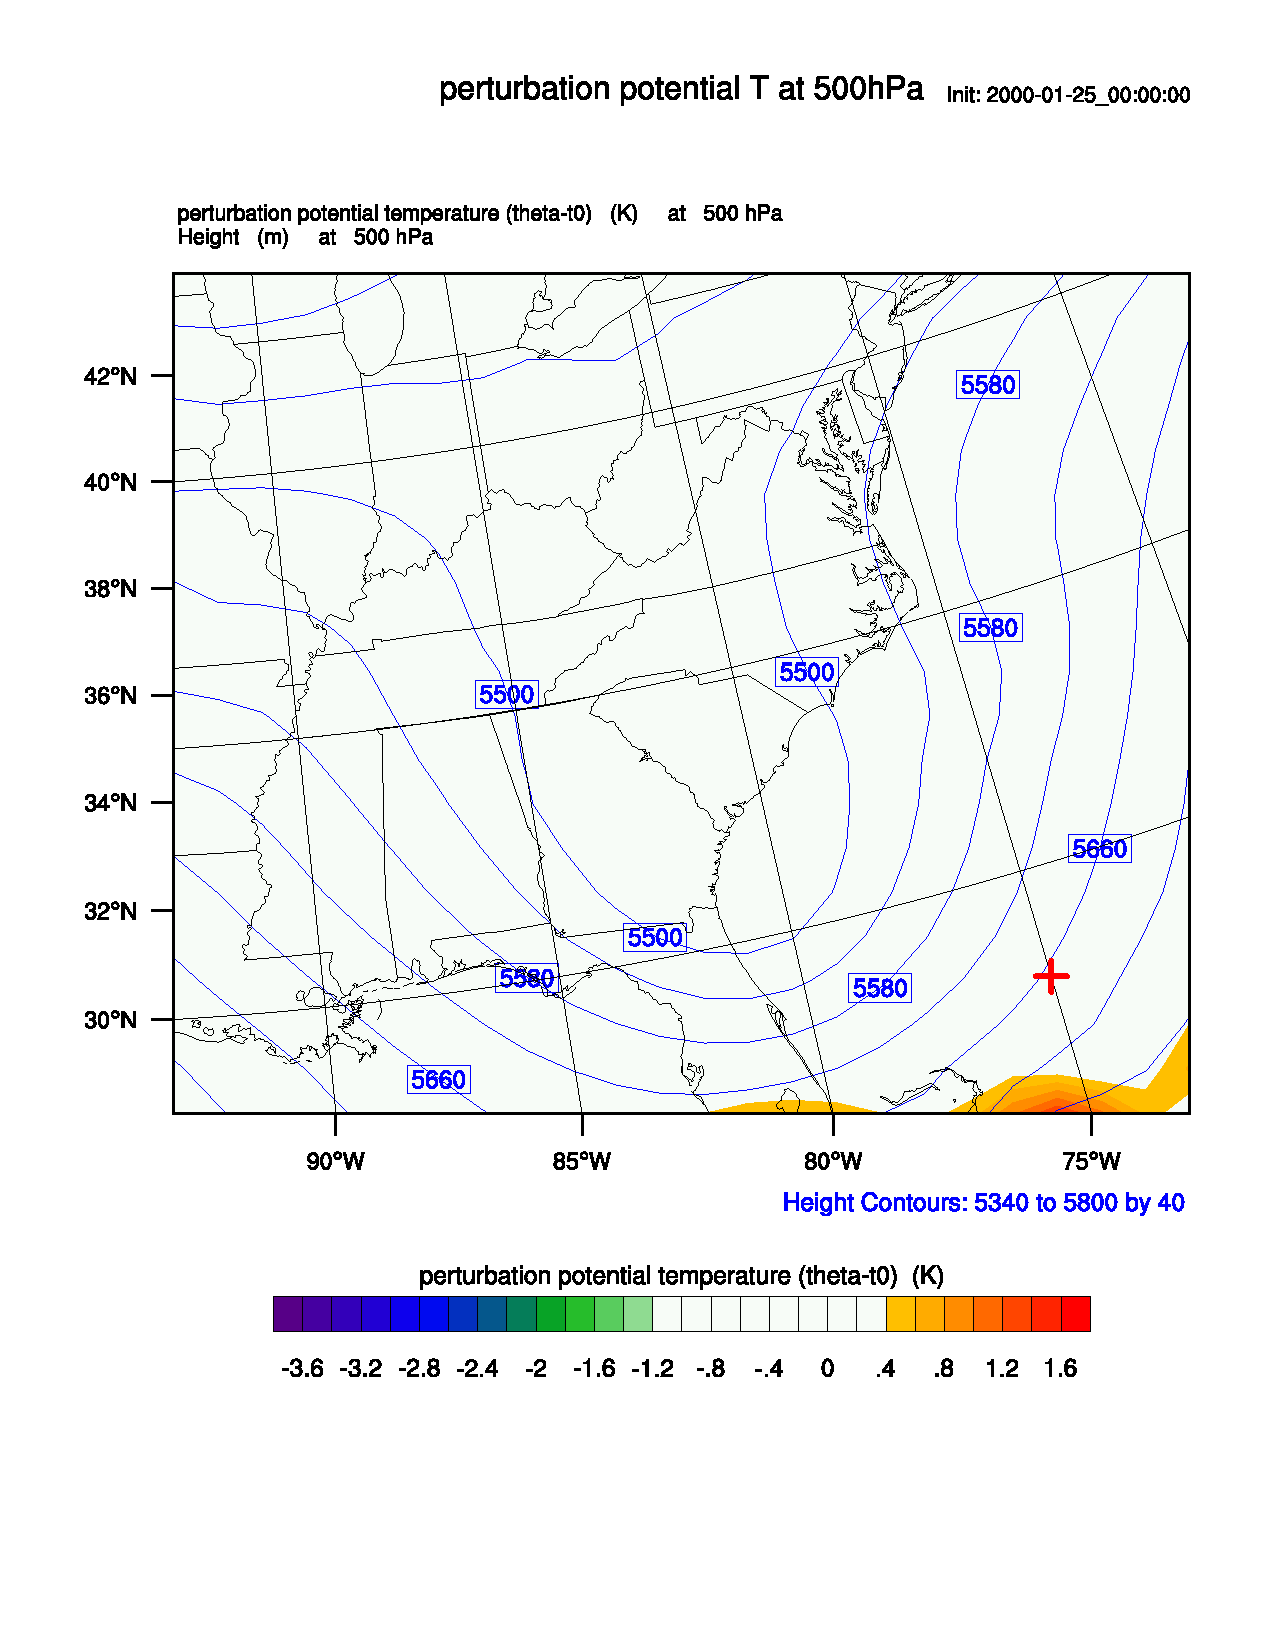
\includegraphics[width=19pc, viewport=40 100 600 730, clip]{./figures/boundary}}
\subfigure[With LBC control]{
\noindent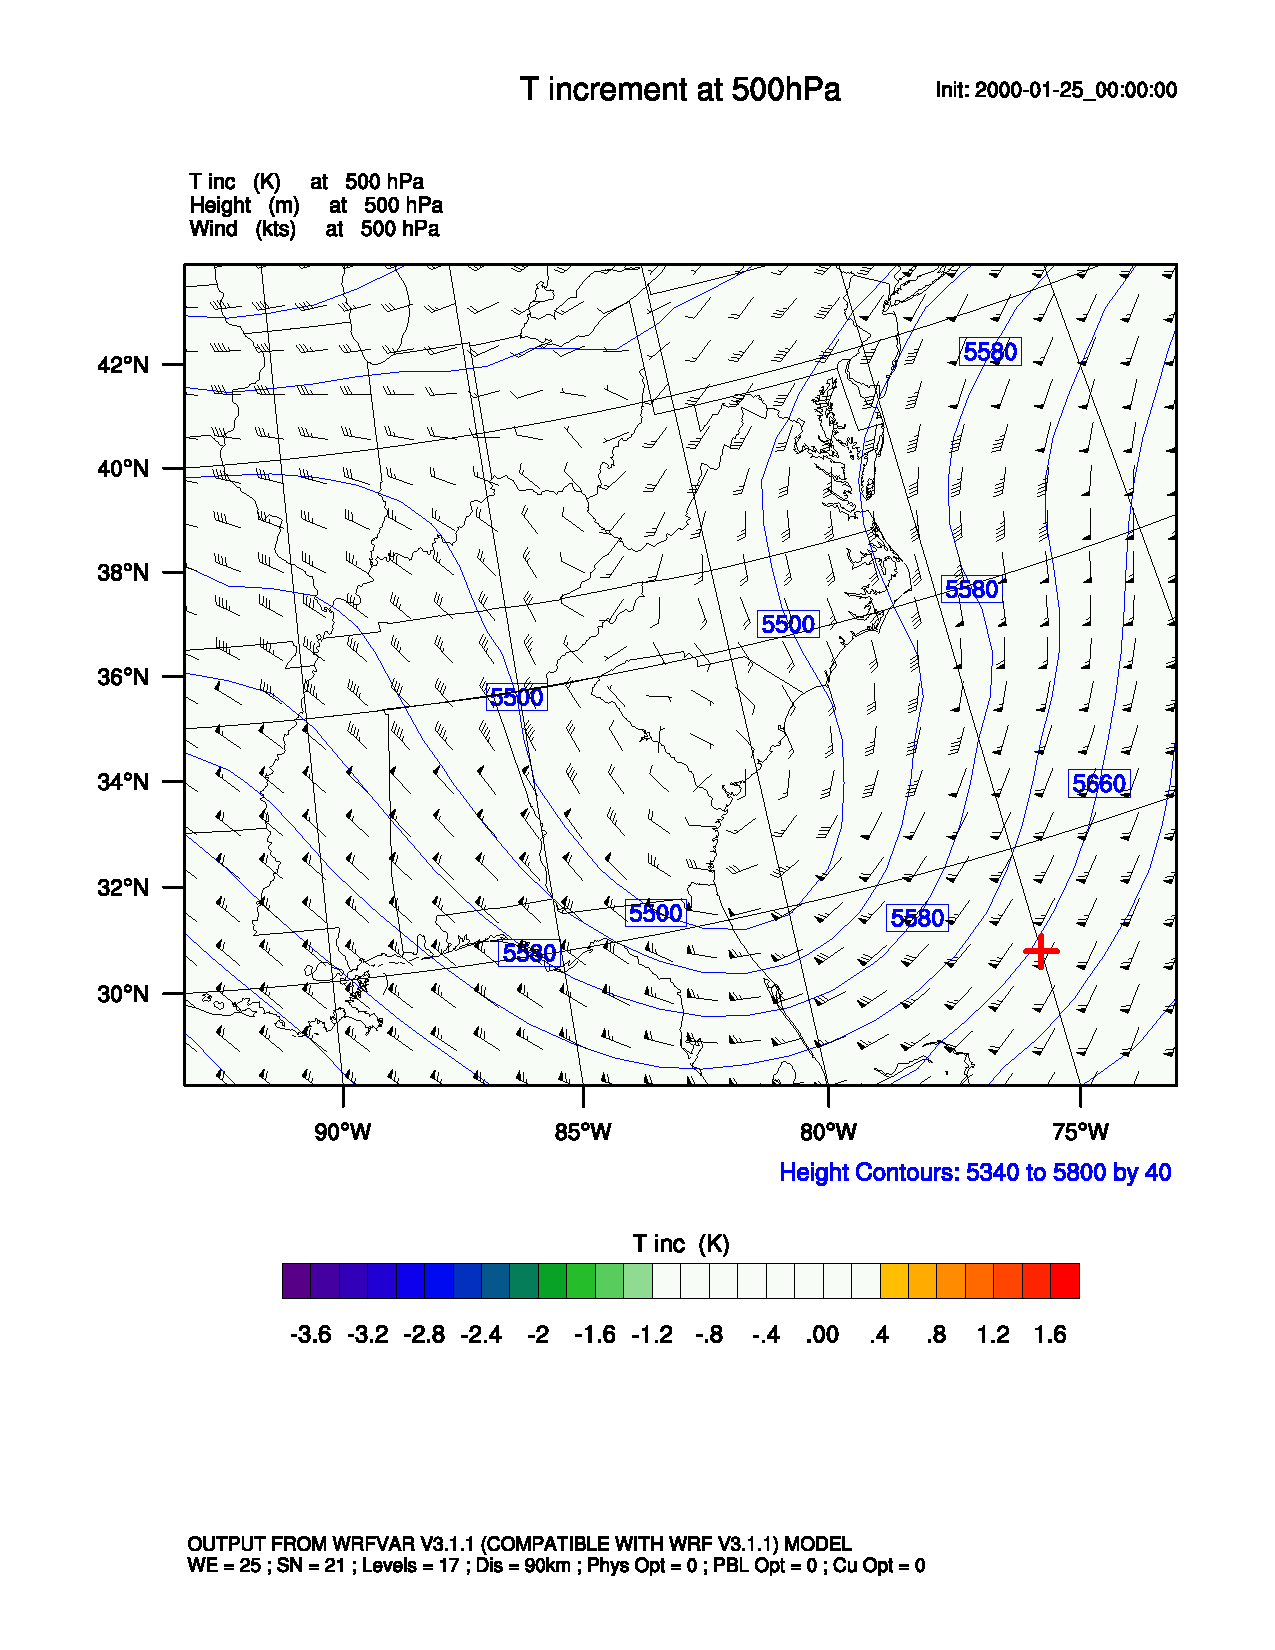
\includegraphics[width=19pc, viewport=40 100 600 730, clip]{./figures/boundary_lbc}}
\caption{0 hour potential temperature perturbation.}\label{fig:boundary_0h}
\end{figure}

\begin{figure}[t]
\begin{center}
\noindent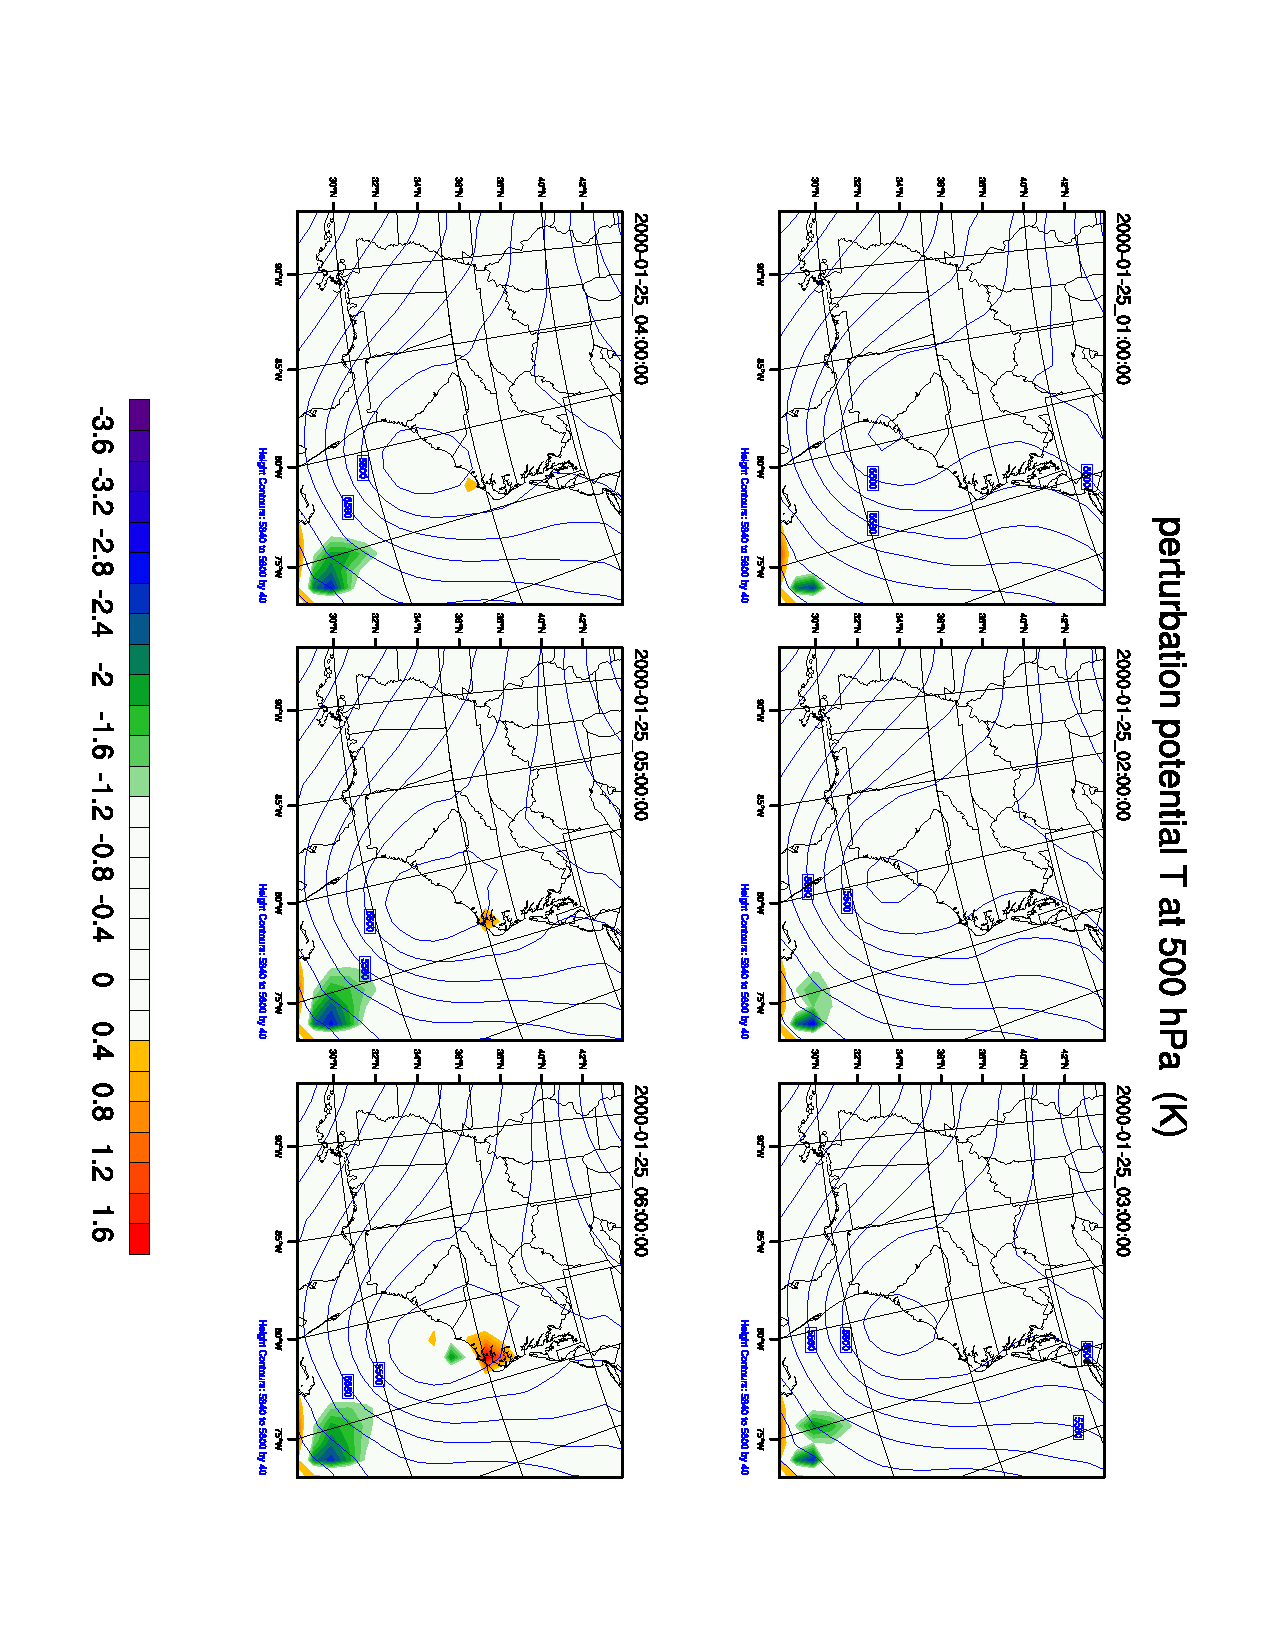
\includegraphics[width=39pc, viewport=20 50 580 750, clip]{./figures/boundary_6h}
\end{center}
\caption{1-6 hour potential temperature perturbation without LBC control.}\label{fig:boundary_6h}
\end{figure}
\begin{figure}[t]
\noindent\includegraphics[width=39pc, viewport=20 50 580 750, clip]{./figures/boundary_lbc_6h}
\caption{1-6 hour potential temperature perturbation with LBC control.}\label{fig:boundary_lbc_6h}
\end{figure}

Above two experiments also confirm the correctness of implementation of the LBC control in minimization.   

\section{Real case}
We randomly pick up the period from April 1 to 5, 2008 of the CONUS domain. The domain size is $43\times31\times28$, grid distance is $135km$. We run the 4D-Var as well as the subsequent 24 hours forecast every 12 hours.

Unlike the single observation experiment, in which the minimization can converge in 1-3 iterations, in real case, there are so many observational data distributed in the three-dimensional model space and along the time window, moreover, the number of iteration of real case is usually more than 50, which will spread the impact of LBC control all over the domain, the impact of LBC control can not be easily identified by the analysis increments as what we did in section \ref{sec:single}.

From the discussion in section \ref{sec:single}, we know that the minimization will produce fake or overestimated analysis increments to fit the downstream observations close to boundary relaxation region if LBC were not include in the minimization. Additionally including LBC in minimization will reduce the fake or overestimated analysis increments in IC, because some of the analysis response due to the observations close to boundary will be redirected to LBC increments.  The IC analysis increments combining with the LBC increments will produce a better observation fitting. In general senses, we could expect that the experiments with LBC control should end with a smaller $J_b$ and $J_o$ than which in experiments without LBC control. Note: This expectation should only be treated as a high probability phenomenon, it is not a definite conclusion since the $J_b$ and $J_o$ are the mixed and together index of the changes of the background.  Table \ref{t1} list the final $J_b$ and $J_o$ in each experiments. The red numbers in Tab. \ref{t1} are two exceptions , all other cases confirm our expectation. Especially, all $J_o$ with LBC control become smaller, which means that during the 6-hour time window, the new model trajectory fits observations better than which without LBC control. 
\begin{table}[t]
\caption{Final $J_b$ and $J_o$ comparison.}\label{t1}
\begin{center}
\begin{tabular}{c|c|c|c|c}
\hline\hline
\multicolumn{3}{c}{$J_b$} \vline & \multicolumn{2}{c}{$J_o$}\\
\hline
Date & w LBC & w/o LBC &  w LBC &  w/o LBC\\
\hline
 1500 & \textcolor{red}{1913} & 1903 & 15326 & 15607 \\
 1512 & 2031 & 2097 & 15904 & 16101 \\
 1600 & 2787 & 2885 & 27237 & 27583 \\
 1612 & 2561 & 2622 & 28084 & 28371 \\
 1700 & \textcolor{red}{3463} & 3458 & 37099 & 37482 \\
 1712 & 2505 & 2590 & 32515 & 32760 \\
 1800 & 2883 & 2911 & 33824 & 34337 \\
\hline
\end{tabular}
\end{center}
\end{table}

Next, we will show the verification scores of the 12 and 24 hour forecast upon the observations. Fig.~\ref{fig:bias_12h}, ~\ref{fig:rmse_12h} and Fig.~\ref{fig:bias_24h}, ~\ref{fig:rmse_24h} are the BIAS and RMSE profiles of the 12 and 24 hours forecast verified against the observations respectively. Basically, the verification results are quite mixed, even the 24 hour V component forecast with LBC control shows some degrade. It is hard to make a definite conclusion of which experiment is better since the period of experiments is very limited. According to the personal communication with the developers of HIRLAM system, the improvement due to the LBC control is very trivial and unnoticeable even in a long time operational parallel experiments. Therefore, long time parallel run is needed to evaluate the impact of the LBC control on the forecast.
\begin{figure}[t]
\begin{center}
\noindent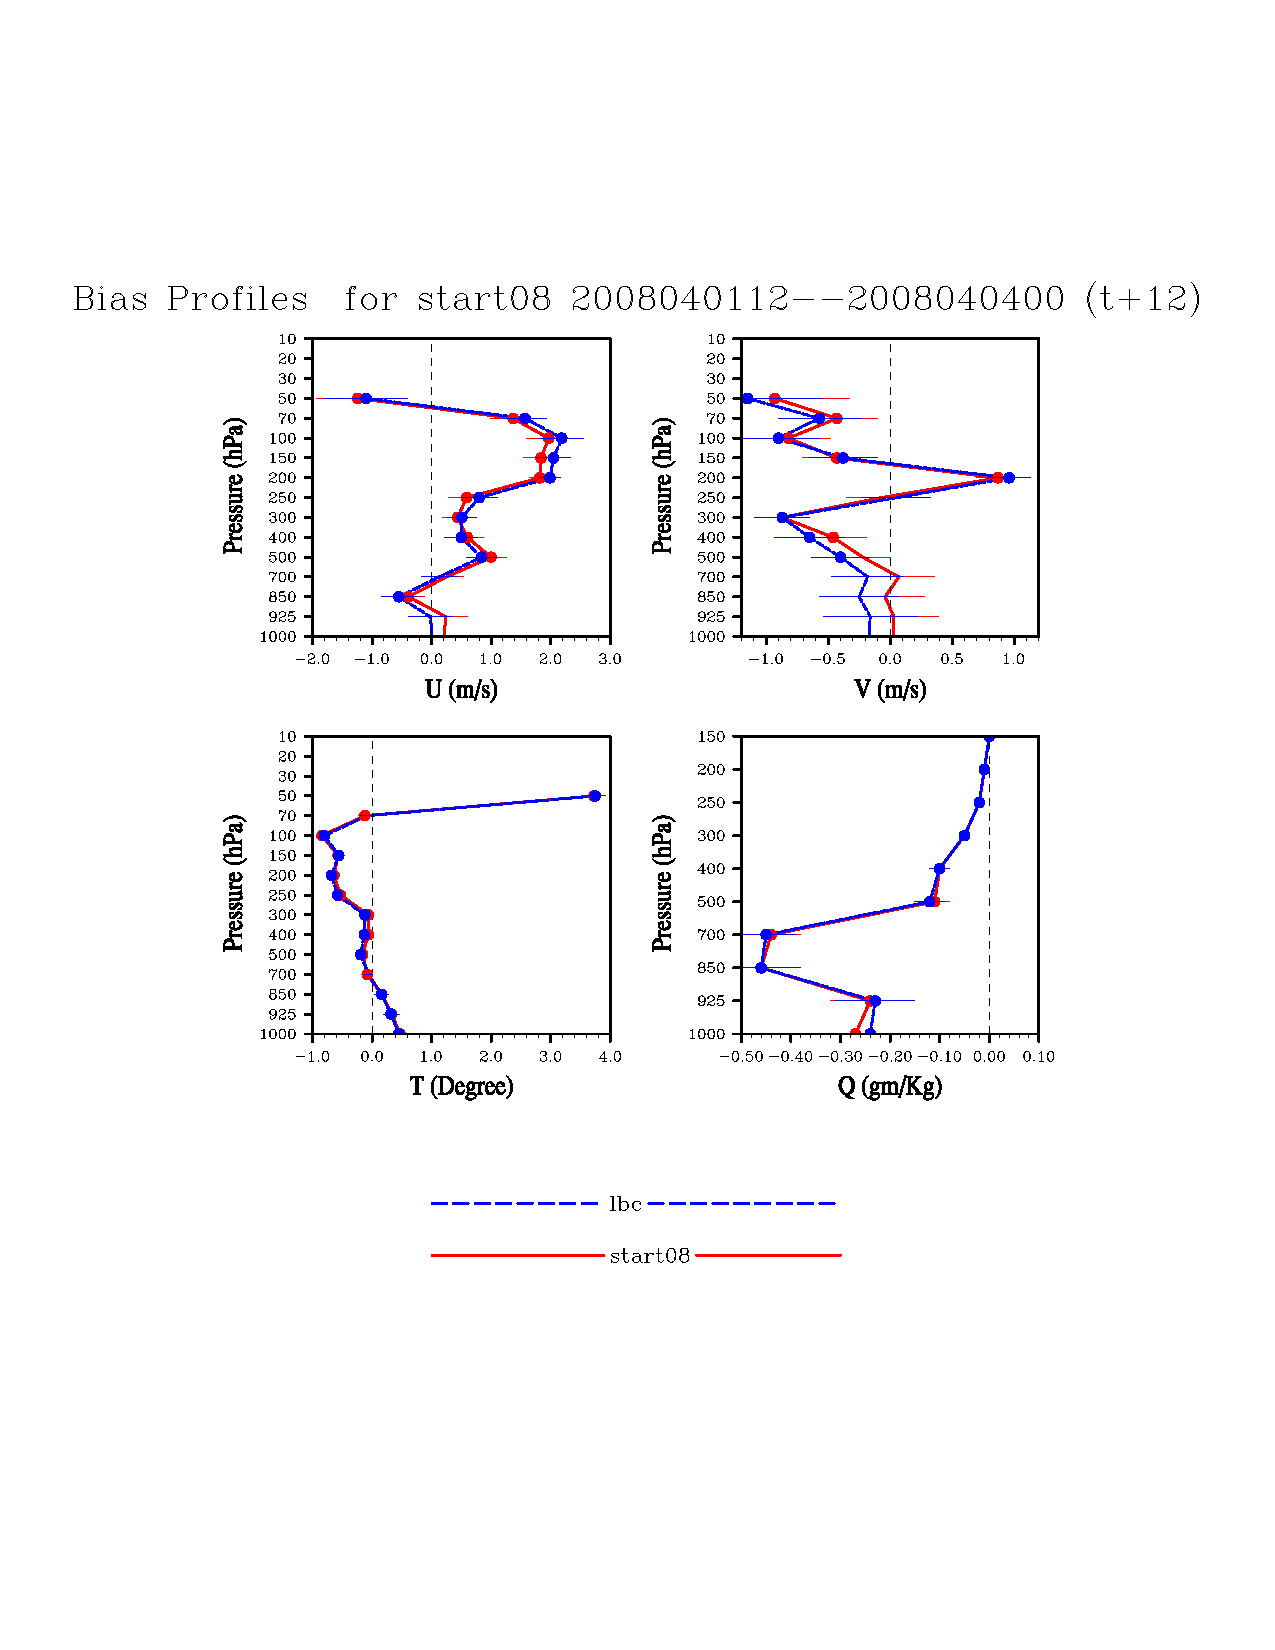
\includegraphics[width=39pc, viewport=20 250 580 750, clip]{./figures/Profile_BIAS_12}
\end{center}
\caption{12 hour bias profiles of forecast verified against observations. \textcolor{blue}{Blue} lines is the experiments with LBC control;  \textcolor{red}{Red} lines is the experiments without LBC control.}
\label{fig:bias_12h}
\end{figure}

\begin{figure}[t]
\begin{center}
\noindent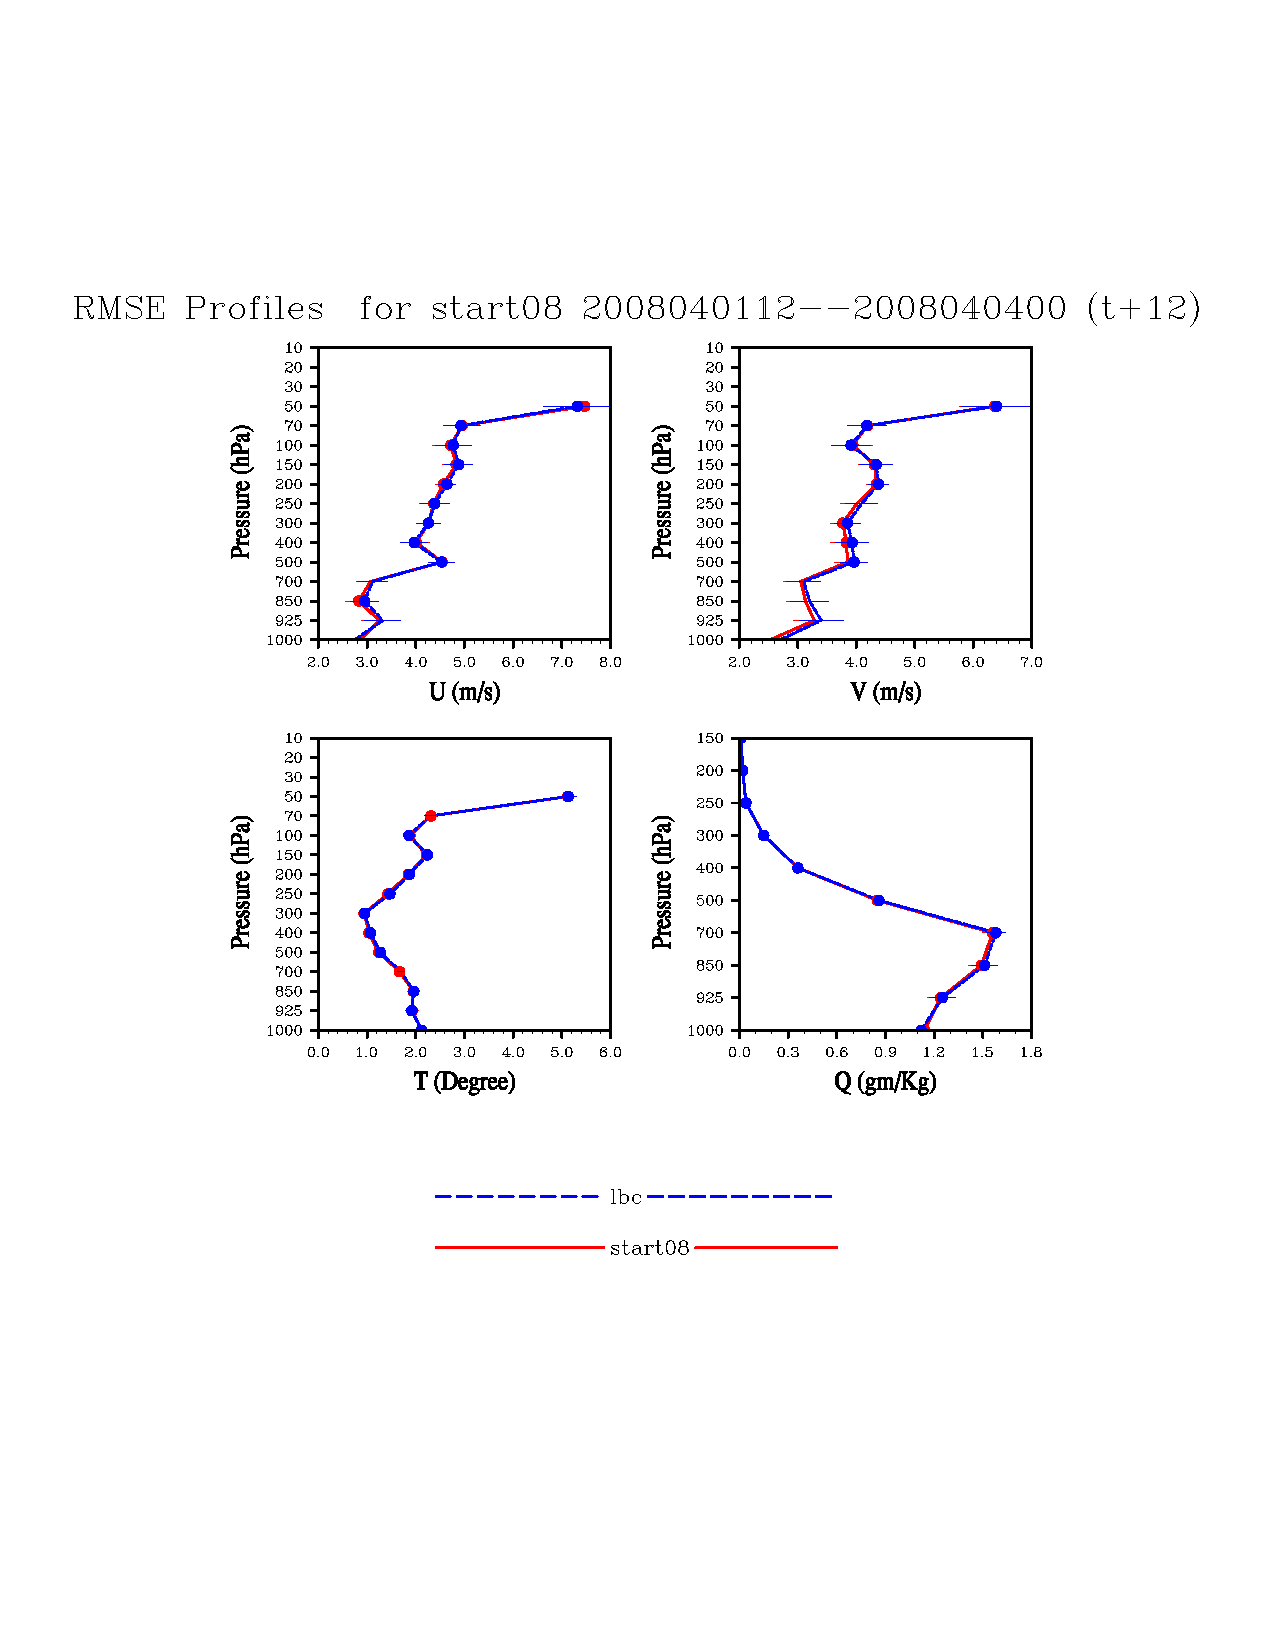
\includegraphics[width=39pc, viewport=20 250 580 750, clip]{./figures/Profile_RMSE_12}
\end{center}
\caption{12 hour RMSE profiles of forecast verified against observations. \textcolor{blue}{Blue} lines is the experiments with LBC control;  \textcolor{red}{Red} lines is the experiments without LBC control.}
\label{fig:rmse_12h}
\end{figure}

\begin{figure}[t]
\begin{center}
\noindent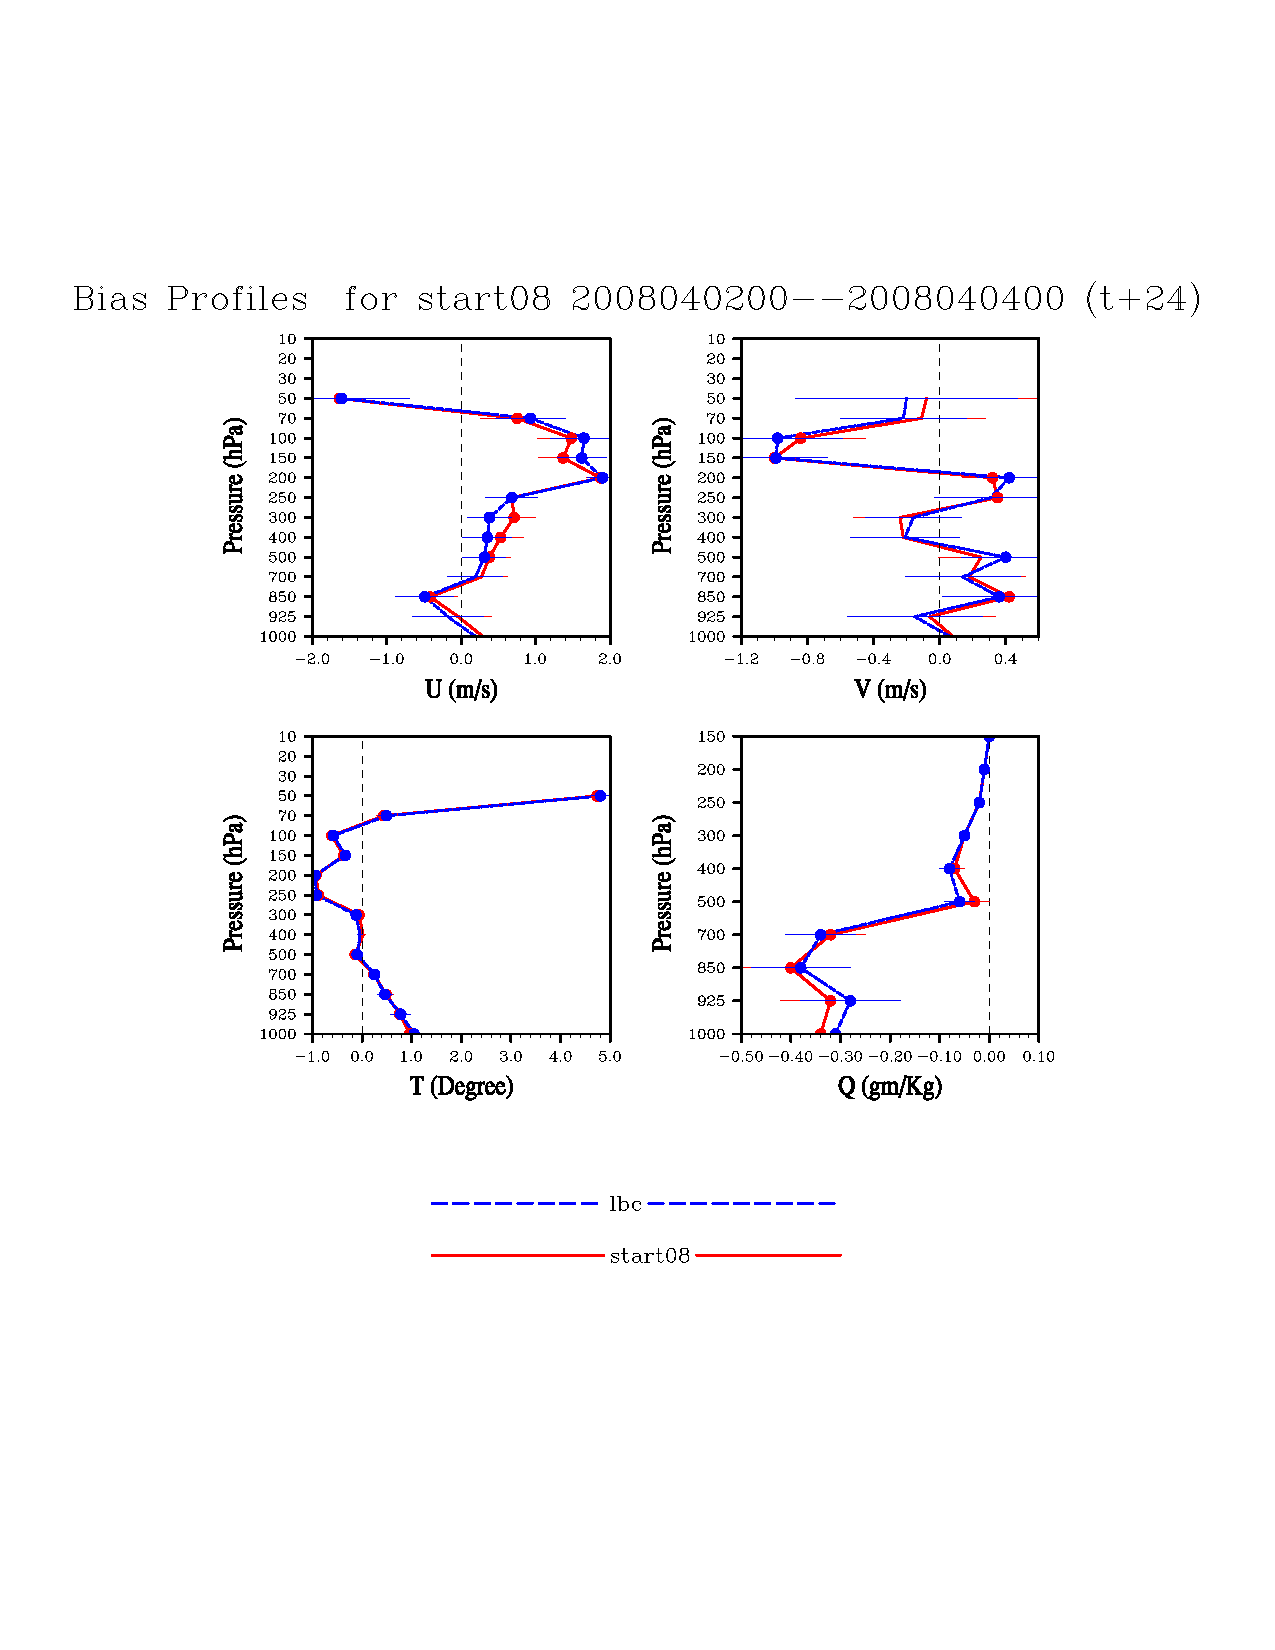
\includegraphics[width=39pc, viewport=20 250 580 750, clip]{./figures/Profile_BIAS_24}
\end{center}
\caption{24 hour bias profiles of forecast verified against observations. \textcolor{blue}{Blue} lines is the experiments with LBC control;  \textcolor{red}{Red} lines is the experiments without LBC control.}
\label{fig:bias_24h}
\end{figure}

\begin{figure}[t]
\begin{center}
\noindent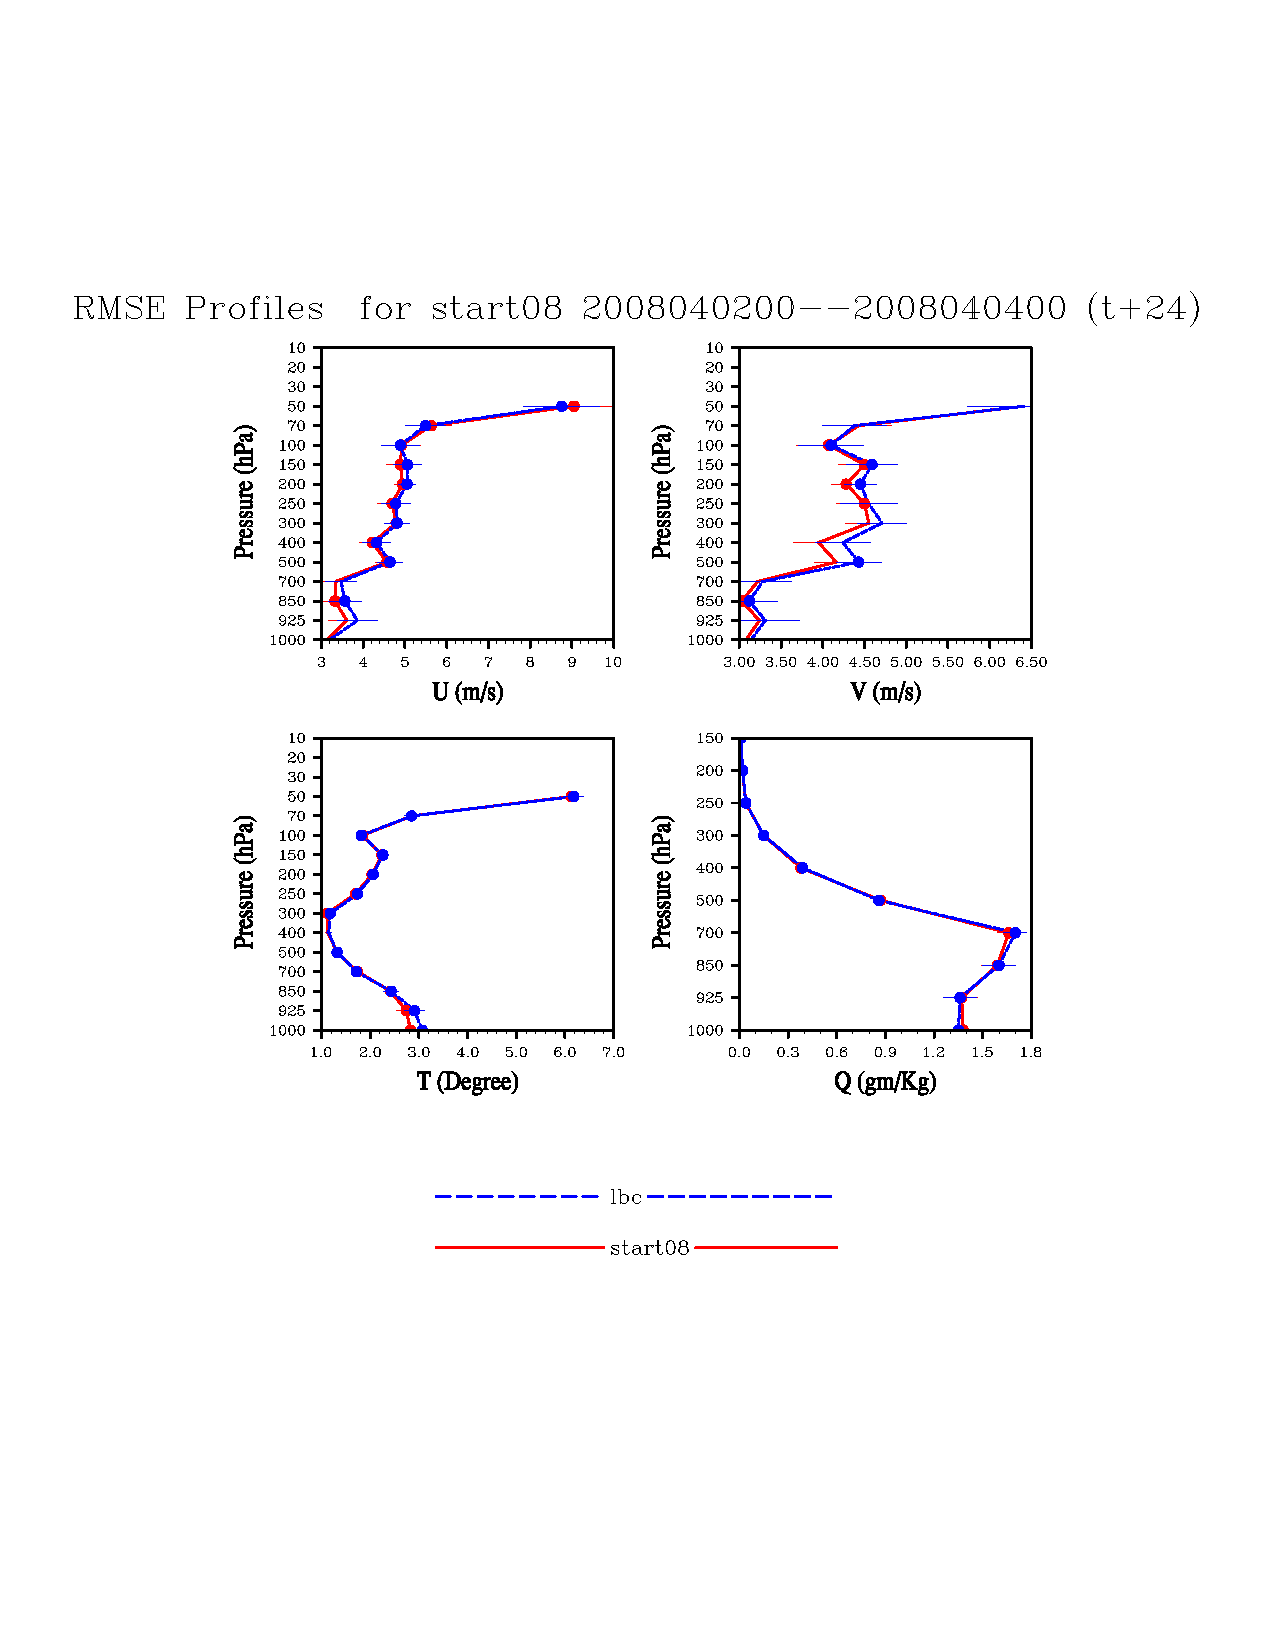
\includegraphics[width=39pc, viewport=20 250 580 750, clip]{./figures/Profile_RMSE_24}
\end{center}
\caption{24 hour RMSE profiles of forecast verified against observations. \textcolor{blue}{Blue} lines is the experiments with LBC control;  \textcolor{red}{Red} lines is the experiments without LBC control.}
\label{fig:rmse_24h}
\end{figure}


\section{Future works}

In current WRF/WRFDA configuration, there is a boundary updating procedure between data assimilation and the subsequent forecast because the data assimilation will changes the initial condition which lead to the changes in the boundary tendency from 0 to 6 hour. Once the LBC of the time window was included in the 4DVar minimization, the tendency of the 0--6 hour LBC  will be updated automatically after the analysis, which also means the state at the end of the time window will be changed too. Then, not only the 0--6 hour LBC tendency should be updated, the 6--12 hour LBC tendency should be updated, this capability should be developed.

%%%%%%%%%%%%%%%%%%%%%%%%%%%%%%%%%%%%%%%%%%%%%%%%%%%%%%%%%%%%%%%%%%%%%
% ACKNOWLEDGMENTS
%%%%%%%%%%%%%%%%%%%%%%%%%%%%%%%%%%%%%%%%%%%%%%%%%%%%%%%%%%%%%%%%%%%%%
\begin{acknowledgment}
The National Center for Atmospheric Research is sponsored by the National
Science Foundation.  This work was supported by the Air Force Weather Agency.
\end{acknowledgment}


%%%%%%%%%%%%%%%%%%%%%%%%%%%%%%%%%%%%%%%%%%%%%%%%%%%%%%%%%%%%%%%%%%%%%
% REFERENCES
%%%%%%%%%%%%%%%%%%%%%%%%%%%%%%%%%%%%%%%%%%%%%%%%%%%%%%%%%%%%%%%%%%%%%
% Create a bibliography directory and place your .bib file there.
\ifthenelse{\boolean{dc}}
{}
{\clearpage}
\bibliographystyle{ametsoc}
\bibliography{../bibliography/references}

\end{document}
%%%%%%%%%%%%%%%%%%%%%%%%%%%%%%%%%%%%%%%%%%%%%%%%%%%%%%%%%%%%%%%%%%%%%
% END OF TEMPLATE
%%%%%%%%%%%%%%%%%%%%%%%%%%%%%%%%%%%%%%%%%%%%%%%%%%%%%%%%%%%%%%%%%%%%%